\section{Understanding the Impact of Proposer Location}
\label{sec:impact}

This section investigates how proposer’s network latency relative to other nodes affects overall consensus performance. We evaluate: (i) the measurable impact on consensus duration; (ii) effects on individual step durations; (iii) influences on quorum formation; and (iv) potential throughput gains using optimized proposer placement. 

We conducted experiments on the CloudLab\footnote{\url{https://cloudlab.us/}} testbed using 13 m510\footnote{\url{https://docs.cloudlab.us/hardware.html\#(part.cloudlab-utah)}} nodes. Each node emulated a distinct AWS zone, with inter-node latencies\footnote{\url{https://github.com/cometbft/cometbft/blob/v2.x/test/e2e/pkg/files/aws-latencies.csv}} injected via the \texttt{tc}\footnote{https://www.man7.org/linux/man-pages/man8/tc.8.html} (traffic control) utility to represent a realistic geo-distributed topology. The study utilized the Malachite implementation of the Tendermint protocol. Each execution lasted five minutes, including a 30-second warm-up and 15-second cool-down, with clock synchronization maintained via NTP to ensure deviations remained below 10ms.

Our experimental methodology followed a sequence of targeted tests. First, a \textit{sanity check} was performed using a 4-node topology with a uniform 100ms latency. The results showed negligible variation ($< 1.6\%$) across proposers, both for fixed and rotating strategies, confirming that any subsequent performance discrepancies were strictly due to network topology.  Also, we observed no impact in switching proposers at each decision or after a number of decisions.  For better legibility, we show figures with results switching proposers every 10 decisions.

\subsubsection{Proposer Impact on Consensus Duration.}
The primary metric for evaluating proposer location is the total time elapsed from the initial proposal to the final decision. In our 13-node heterogeneous topology, we observed that the physical location of the proposer is a dominant factor in system performance. As illustrated in Figure \ref{Idur}.a, consensus durations measured at proposers range from a minimum of 0.47s to a maximum of 0.73s depending on which node lead the round, a 40\% performance gap.   Figure \ref{Idur}.b depicts the latency from proposal to decision as measured at each node, showing that impact on termination latency at each node is also impacted by the proposer.
%demonstrates that even without computational bottlenecks, the network's "center of gravity" significantly dictates the speed of the entire system.

\begin{figure}
     \centering
     \begin{subfigure}{0.95\textwidth}
         \centering
         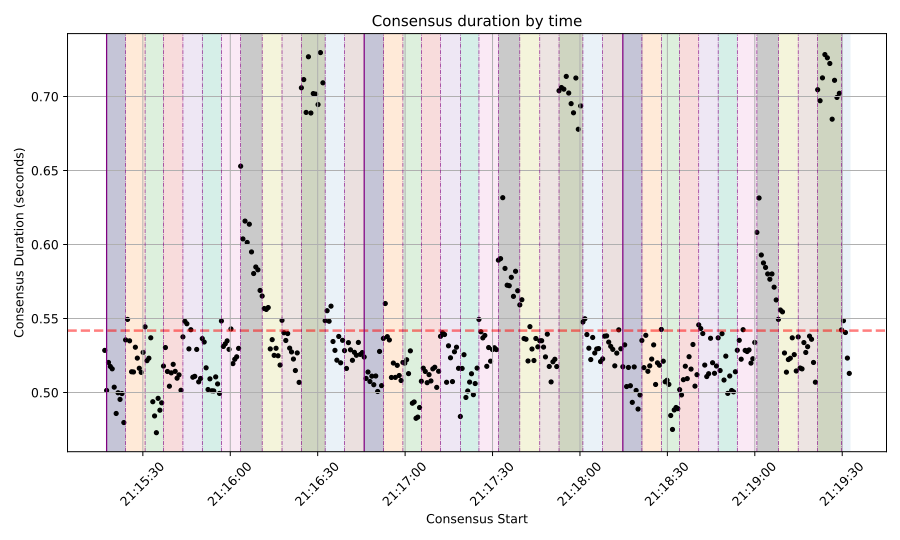
\includegraphics[width=\linewidth]{svgi/10xconsensusDurationLeader.svg.png}
         %\includesvg[width=\linewidth]{svg/10xconsensusDurationLeader.svg}
         \caption{Latency from propose to decide measured at each proposer}
         \label{fig:1a}
     \end{subfigure}
     \\
     \begin{subfigure}{0.95\textwidth}
         \centering
         % Cor nas linhas, ruim de ver de longe
         %\includesvg[width=\linewidth]{svg/10xoptdecidedDeviationBlocktimeLeader.svg}
         %\includesvg[width=\linewidth]{svg/10xoptbackdecidedDeviationBlocktimeLeader.svg}
         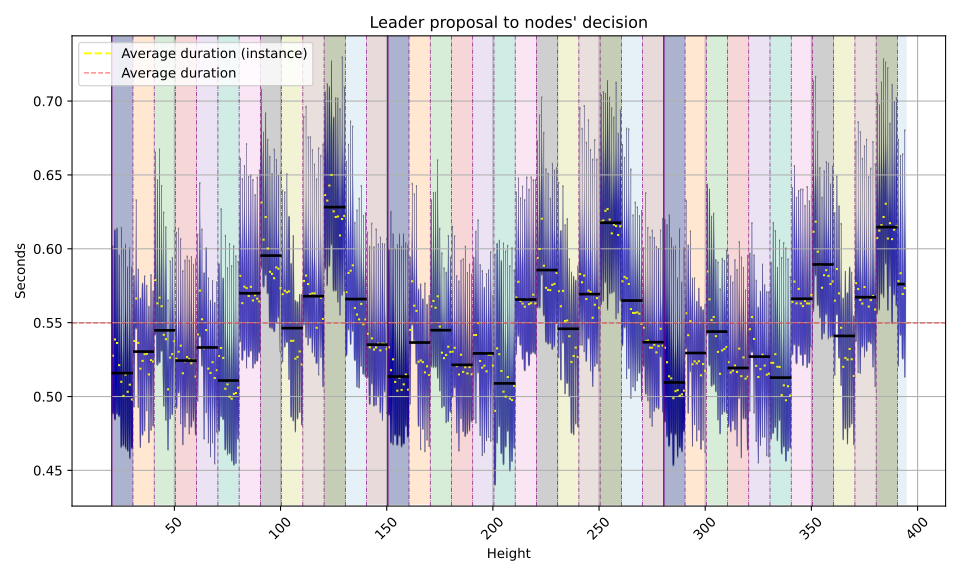
\includegraphics[width=\linewidth]{svgi/10xoptbackdecidedDeviationBlocktimeLeader.svg.png}
         \caption{Each vertical line refers to
a consensus instance and is composed by plots with the consensus latency of each node}
         \label{fig:1b}
     \end{subfigure}
     \caption{(a) Consensus latency at proposer and (b) Consensus latency at all nodes.
     10 instances per proposer, divided by vertical dotted lines. Solid line indicates a new round through same proposers - repeating the pattern, each proposer has a different color. }
     \label{Idur}
\end{figure}

CDF da figura 1.a

cdf da figura 1.b

figura 2 -  nao se justifica

titulo p 4

tail latency nos resultados



\subsubsection{Proposer Impact on Consensus Steps.}
After the proposal, further communication steps are all-to-all. While the time to receive a quorum, in all-to-all communication phases, theoretically depends on the location of each receiver node, 
%in proposer-based algorithms are theoretically symmetric, 
we investigated whether the proposer's location could influence such steps.
%We define \textit{prevote} duration as the interval from proposal receipt to quorum collection, and \textit{precommit} duration as the time from prevote quorum to precommit quorum.
%
Fig.\ref{fig.steps} displays individual prevote (a) and precommit (b) step durations, showing that proposer location measurably also impacts the latency of these consensus phases.   

\begin{figure}
     \centering
     \begin{subfigure}{0.95\textwidth}
         \centering
         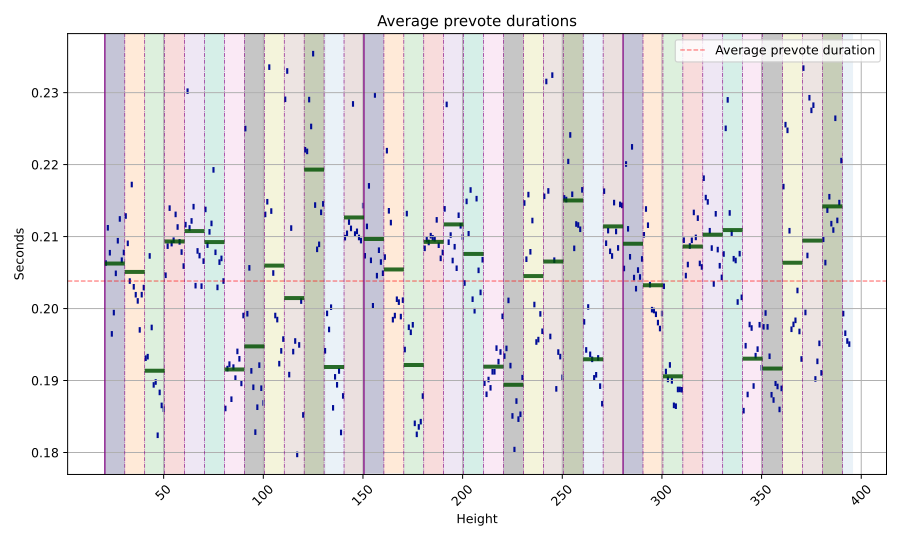
\includegraphics[width=\linewidth]{svgi/10xlimStepPrevoteLeader.svg.png}
         \caption{}
         \label{fig:2a}
     \end{subfigure}
     \\
     \begin{subfigure}{0.95\textwidth}
         \centering
         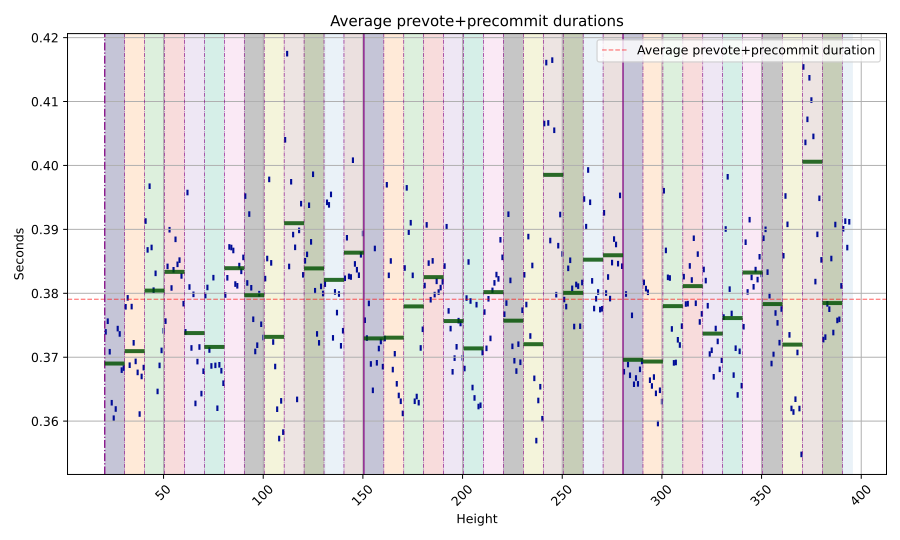
\includegraphics[width=\linewidth]{svgi/10xlimStepPrevotePrecommitLeader.svg.png}
         \caption{}
         \label{fic:2b}
     \end{subfigure}
     \caption{(a) For each instance a we measure each nodes latencies from receiving a proposal until a quorum of prevotes is received. We then calculate the per-proposer mean (green) and global mean (red).  \\
     (b) The same for each nodes latencies from receiving the proposal until a quorum of precommits is received.}
     \label{fig.steps}
\end{figure}


\subsubsection{Influences on Quorum Formation.}
One hypothesis to better understand the previous result is that 
a proposer impacts the formation of quorums, which in turn affects step durations.
%Suppose a proposer $p$ close to a node $n_1$, which is distant from $n_2$.  $n_1$ would quickly respond $p$'s $propose$ message with $prevote$ to all nodes, possibly reaching $n_2$ before other nodes messages to $n_2$, i.e. $n_2$'s prevote quorum includes a distant node $n_1$. 
To check this, we computed and evaluated the quorums built at each node, rotating the whole set of proposers several rounds.   We observed a 98\% consistency in quorum composition when the same node acted as proposer. Nodes geographically closer to the proposer receive the proposal faster and, consequently, their votes are the first to arrive and form the $prevote$ quorum.
%
As stated in the Tendermint specification, if a farther node manages to join another node’s prevote quorum, that second node will wait for that node in the $precommit$ step even if a faster quorum is reached (this is intended for Proof of Stake rewards).   This means that in the precommit phase, a specific node cannot progress with it's ideal quorum (set of closest nodes), negatively impacting latency and throughput.   This also leads to the high consistency among prevote and precommit quorums in a specific node.

\subsubsection{Throughput Gains via Proposer Placement}
The final aspect of our analysis compared the standard round-robin rotation against a fixed-proposer configuration using topologically "ideal" nodes. The results confirm that by steering the protocol to favor leaders with lower median latency to the rest of the network, the system achieves significantly higher sustained throughput.

 [??? bla bla ... tem que colocar numeros aqui !!!!  e fazer o texto mais sucinto ]

This gain is achieved without modifying the underlying BFT safety logic, proving that performance-aware leader selection is a viable optimization for geo-distributed blockchains.

